\section{Introduction}

\subsection{Installation}

Find this documentation
and the scripts it refers to
at \code{github.com/stefantkeller/VECSELsetup}.
From within the EPFL network
find a VECSEL starter-kit
with the relevant manuals and publications
to start with
at \code{wiki.epfl.ch/vecsel-lpn/documents/VECSEL-starterkit.zip}.

This is a Python library.
If you don't have Python installed yet,
I recommend you install ``Anaconda'' (\code{http://continuum.io/downloads})
for Python 2.7 (it's free!).
Also,
you have to have installed
the drivers from National Instrument (\code{ni.com}),
in order to communicate with GPIB
(etc\ldots (NI drivers are a mess, what exactly you need, you have to figure out yourself)).

To install this library
from github,
\begin{enumerate}
  \item click on ``Download ZIP'',
  \item extract the .zip
  \item copy the folder to where ever you want it
  \item adjust the PYTHONPATH
\end{enumerate}
(at least, that's the proper way to do it, I guess).  
And, if you are familliar with git \ldots you know what to do.

If you don't care about ``proper''
and you simply want it to work
(I don't know though what this breaks along the way\ldots):  
after extracting the .zip,
copy the folder to (something like; if you work with Anaconda as recommended above)
\begin{itemize}
  \item Windows: \code{C:\textbackslash Anaconda\textbackslash Lib\textbackslash site-packages}
  \item Mac: \code{/Users/yourusername/anaconda/Lib/python2.7/site-packages}
\end{itemize}
this path is already in the Pythonpath,
and Python will find it.

For measurements (the stuff in \code{meas/}) you need pyvisa \\
(\code{https://pyvisa.readthedocs.org/en/master/}).\\
For evaluation (the stuff in \code{eval/}) you need to also install errorvalues \\
(\code{https://github.com/stefantkeller/errorvalues}). \\
Install it with the same procedure as listed above.
If you intend to use the calibration in \code{exp/eval/calibration.py} as it is,
this is going to write an automated report (tuck together some plots) as a pdf;
ready for print.
This relys on \LaTeX (\code{pdflatex}) to be installed on your system.

If measurement and evaluation happens on two different computers (recommended)
you probably install only those dependencies that you need.
That's ok, the error handling in \code{\_\_init\_\_.py}
catches \code{ImportError}s and ignores them.
However, if nothing happens at all,
you might want to check whether you have installed,
what you're supposed to have installed
(maybe everything is caught and subsequentially ignored?).

\subsection{File hierarchy}

The different folders have different purposes:
\begin{itemize}
  \item meas, setup control to record measurements
  \item eval, scripts for evaluation of measurements
  \item exp, examples of working measurement routines (using meas), and evaluation (using eval)
  \item doc, documentation
\end{itemize}

\subsection{Usage}

Copy the files stored from the folder \code{exp} in your working directory.
The example \code{exp/meas/routine\_measurement.py} is the most exhaustive for setup control / recording measurements.
While \code{exp/eval/light\_light.py} highlights the evaluation part.

There is not graphical user interface (GUI),
as one might know from LabView.
Instead, with this library
you have full controll over
what the software does.
But this comes with the price
to actually having to read the lines of code --
instead of looking at obscure icons.
There are only few lines of code
to read,
in order to understand what's going on;
and those are accompanied with comments.
So go ahead and read it.
You best start with the example scripts in the folder \code{exp}.

These lines of code
you can read with any text editor
of your choosing.
On Windows I recommend PyScripter (\code{https://code.google.com/p/pyscripter/}).
It brings in some simple GUI features,
so you can edit and launch your measurement routines easily,
see Fig.~\ref{img:pyscripter}.

Additionally:
consider TeamViewer \code{teamviewer.com}
as a means to access the lab computer
remotely from your office.

\begin{figure}
\centering
\subfigure{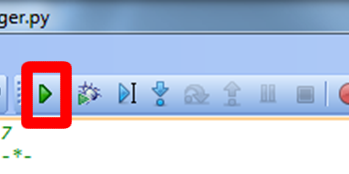
\includegraphics[width=4cm]{img/pyscripter_launch.png}}
\subfigure{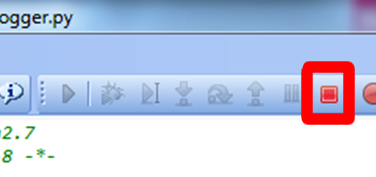
\includegraphics[width=4cm]{img/pyscripter_stop.png}}
\subfigure{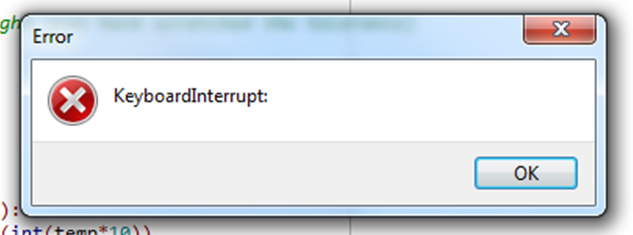
\includegraphics[width=4.5cm]{img/pyscripter_ki.png}}
\caption{PyScripter is a convenient tool
to work with python scripts.
When you have opened one of the examples
from the folder \code{exp/}
you can simply click on the launch button,
the scripts starts and
writes the output in one of the subwindows --
try it out, should be selfexplanatory.
The stop button
lets you to interrupt the script if required.
For example, \code{exp/meas/temp\_logger.py}
logs the heat sink temperature in an infinite loop;
in order to stop the logging you have to interrupt it.
This interruption raises a \code{KeyboardInterrupt} error.
This is supposed to happen.}
\label{img:pyscripter}
\end{figure}

\subsection{Disclaimer}

Some paragraphs in this documentation
are copy-paste from the master project report,
during whose period the presented scripts
have established themselves.
A back-up copy of said report
you will find at \\
\code{github.com/stefantkeller/VECSELMasterProjectReport}.
